\documentclass {article} 
\usepackage{graphicx}
\usepackage [14pt]{extsizes}
\usepackage{xcolor}
\usepackage{wasysym}
\usepackage{amsmath}
\usepackage{amssymb}
\usepackage{asymptote}
\usepackage[russian]{babel}
\title{test 2}
\author{varvara samsonova}
\date{\today}
\begin{document}
\maketitle
\tableofcontents
\section{Images}
\begin{figure}
\centering
\begin{minipage} {0.45\textwidth}
    \centering
        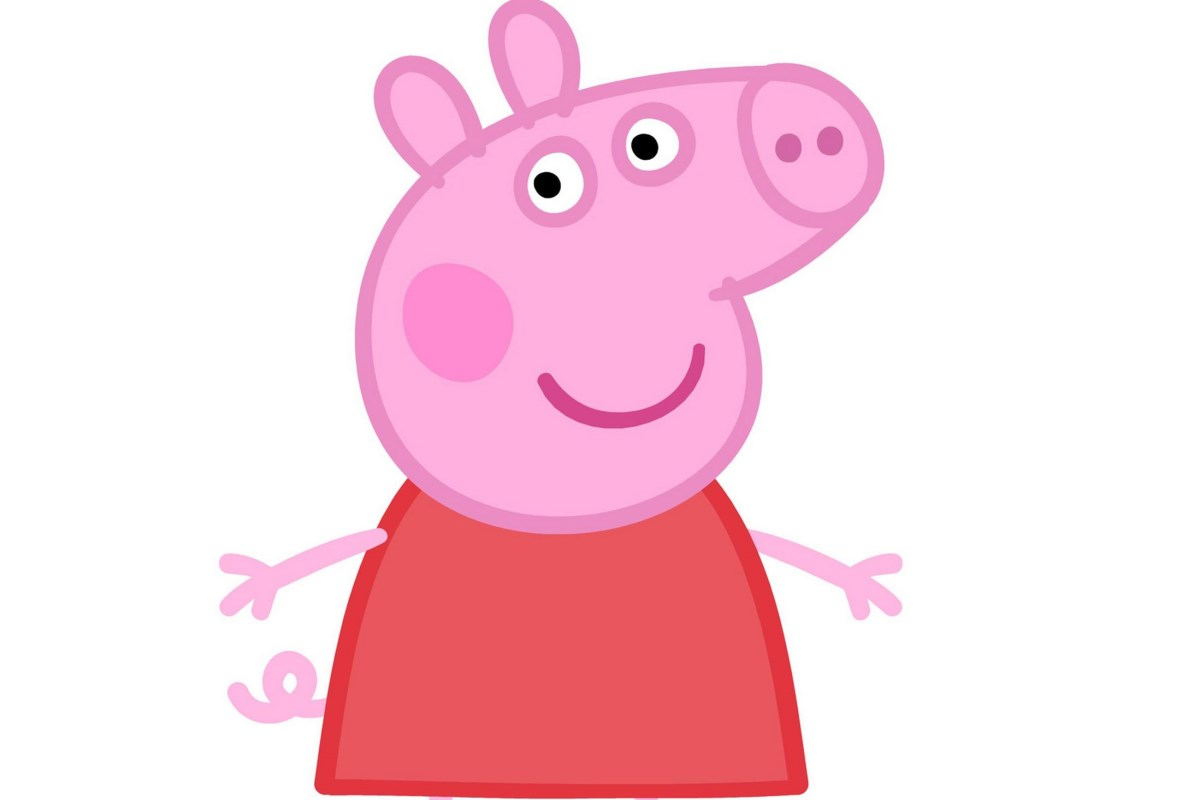
\includegraphics[width=0.9\textwidth]{image.png}
            \caption{свинк пепп}
    \end{minipage}\hfill
    \begin{minipage} {0.45\textwidth}
    \centering
    \begin{asy}
settings.outformat="pdf";
size(2cm);
path thebox = box((0,0),(1,1));
fill(thebox, blue);
draw(shift(.5,.5)*thebox,green+linewidth(5pt));
clip(thebox);
draw(shift(-.5,-.5)*thebox,red+linewidth(5pt));
\end {asy}
\caption {асимптота}

\end{minipage}
\end{figure}

\end{document}